A raiva � uma doen�a viral e infecciosa, transmitida por mam�feros. A campanha nacional de vacina��o antirr�bica tem o objetivo de controlar a circula��o do v�rus da raiva canina e felina, prevenindo a raiva humana. O gr�fico mostra a cobertura (porcentagem de vacinados) da campanha, em c�es, nos anos de 2013, 2015 e 2017, no munic�pio de Belo Horizonte, em Minas Gerais. Os valores das coberturas dos anos de 2014 e 2016 n�o est�o informados no gr�fico e deseja-se estim�-los. Para tal, levou-se em considera��o que a varia��o na cobertura de vacina��o da campanha antirr�bica, nos per�odos de 2013 a 2015 e de 2015 a 2017, deu-se de forma linear.

\begin{figure}[h]
\centering
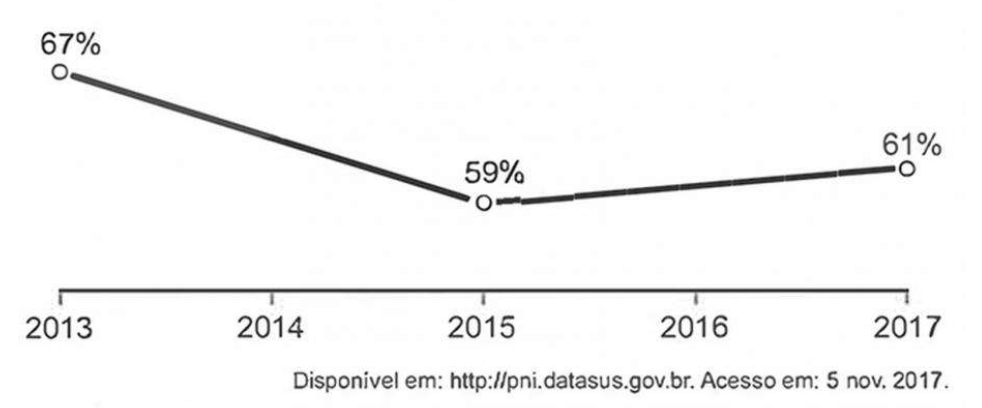
\includegraphics[width=8cm]{../figuras/q152-2018}
\end{figure}

Qual teria sido a cobertura dessa campanha no ano de 2014?

\begin{enumerate}
\item[a)]63,3\%
\item[b)]63,0\%
\item[c)]63,5\%
\item[d)]64,0\%
\item[e)]65,5\%
\end{enumerate}